\documentclass[fontset=none]{ctexart}

\usepackage[T1]{fontenc}
\usepackage{fontspec}
\setCJKmainfont{SimSun}
% Latin Modern
\renewcommand*\ttdefault{txtt} % 改等宽字体

\setcounter{tocdepth}{5}
\setcounter{secnumdepth}{5}
% -1 part
% 0 chapter
% 1 section
% 2 subsection
% 3 subsubsection
% 4 paragraph
% 5 subparagraph

\usepackage{cite}
\usepackage{geometry}
\geometry{a4paper,scale=0.8}

\usepackage{algorithm}  
\usepackage{algorithmicx}  
\usepackage{algpseudocode}
\makeatletter
\newenvironment{breakablealgorithm}
  {% \begin{breakablealgorithm}
   \begin{center}
     \refstepcounter{algorithm}% New algorithm
     \hrule height.8pt depth0pt \kern2pt% \@fs@pre for \@fs@ruled
     \renewcommand{\caption}[2][\relax]{% Make a new \caption
       {\raggedright\textbf{\ALG@name~\thealgorithm} ##2\par}%
       \ifx\relax##1\relax % #1 is \relax
         \addcontentsline{loa}{algorithm}{\protect\numberline{\thealgorithm}##2}%
       \else % #1 is not \relax
         \addcontentsline{loa}{algorithm}{\protect\numberline{\thealgorithm}##1}%
       \fi
       \kern2pt\hrule\kern2pt
     }
  }{% \end{breakablealgorithm}
     \kern2pt\hrule\relax% \@fs@post for \@fs@ruled
   \end{center}
  }
\makeatother

\usepackage{amsmath}
\usepackage{amssymb}
\usepackage{graphicx}
\usepackage{subfigure}
\usepackage{changepage}
\usepackage{multirow}
\usepackage{url}

\usepackage{amsthm}
\newtheorem{theorem}{Theorem}[section]
\newtheorem{lemma}[theorem]{Lemma}
\newtheorem{proposition}[theorem]{Proposition}
\newtheorem{corollary}[theorem]{Corollary}
% \newtheorem{remark}{Remark}[section]
\newtheorem{example}{Example}[section]
\newenvironment{solution}{\begin{proof}[Solution]}{\end{proof}}
\theoremstyle{definition}
\newtheorem{definition}{Definition}[section]
\theoremstyle{remark}
\newtheorem*{remark}{Remark}

\usepackage[colorlinks, linkcolor=black, citecolor=blue, bookmarksnumbered]{hyperref}
% \hypersetup{
% 	colorlinks=true,
% 	linkcolor=cyan,
% 	filecolor=blue,      
% 	urlcolor=red,
% 	citecolor=green,
% }

\usepackage{fancyhdr}
\pagestyle{fancy}
\renewcommand{\sectionmark}[1]{\markright{\thesection\ #1}}
\fancyhf{}
\cfoot{\thepage}
\lhead{\rightmark}
% \rightmark 当前的节名
% \leftmark 当前的章名
% \(l/c/r)head{}, \(l/c/r)foot{}
\renewcommand{\headrulewidth}{0.4pt}
\renewcommand{\footrulewidth}{0pt}

\renewcommand\refname{References}
\renewcommand\contentsname{Contents}
\renewcommand\figurename{Figure}
\renewcommand\tablename{Table}

\begin{document}

\begin{titlepage}
    \begin{center}
        \vspace*{1cm}
            
        \Huge
        \textbf{Traffic State Prediction\\Based On Road Correlation Analysis\\With GPS Data}
            
        \vspace{0.5cm}
        \LARGE
        Mid Report\\
            
        \vspace{1.5cm}
            
        \textbf{11812804}\quad 董正\\

        \vspace{0.5cm}
        Supervisior: 宋轩
            
        \vfill
            
        
\includegraphics[width=\textwidth]{images/sustc.png}
            
        \vspace{0.2cm}
            
        \Large
        Department of Computer Science and Engineering\\
        \vspace{0.5cm}
        Mar. 2022
            
    \end{center}
\end{titlepage}

\tableofcontents

\clearpage
\section{Preliminaries}
\subsection{Introduction}

With the great development of modern cities, the rapid growth of population and the acceleration of urbanization
has made transportation systems to an essential infrastructure. And Transportation systems are becoming more and more
complex, which causes great pressure on urban traffic management.\cite{yin2021deep}

Modern transportation systems contain road vehicles, railway transportation and a variety of newly emerged
shared travel modes, including online ride-hailing, bike-sharing, etc.. In order to alleviate transportation related
problems and manage the expanding transportation systems efficiently, 
traffic prediction or traffic forecasting is brought up by researchers in recent years.

Traffic forecasting is typically based on consideration of historical traffic state data.
In the development of intelligent transportation systems, traffic states are detected by traffic sensors,
bus and metro transactions logs, traffic surveillance cameras and GPS device data.
However, traffic state data is hard to manage because it involves large data volumes with high dimensionality.
Its typical characteristic is that it contains both spatial and temporal domains.
The traffic state in a specific location has both spatial dependency, which may not
be affected only by nearby areas, and temporal dependency, which may be seasonal.
Traditional time series prediction models cannot handle such spatiotemporal prediction problems.
Therefore, deep learning methods have been introduced in this area.\cite{jiang2021graph}
\begin{figure}[htb]
  \centering
  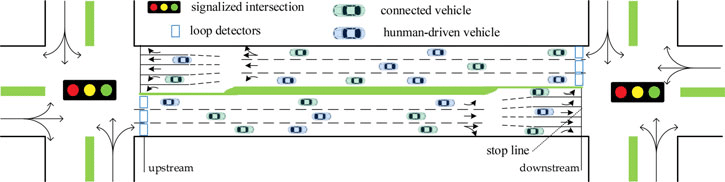
\includegraphics[width=\textwidth]{images/mid/1-1.png}
  \caption{Road Traffic System\cite{yao2020dynamic}}
  \label{1-1}
\end{figure}

\subsection{Motivation}
Figure \ref{fig: 1-2} shows the workflow of traffic prediction procedure.
Then we focus on the data organization of the model's input.
As shown in figure \ref{fig: 1-3}, we first match a GPS sequence into a trajectory,
i.e. a series of roads, then sum the corresponding flow of each road. 
After that, we will get a flow matrix with time as x-axis and road ID as y-axis.
Logically it is just stack the road network's flow vector by time.

\textbf{Almost every state-of-the-art GNN models use stacked vector\cite{lee2021short} as input.
However, this kind of stacked vector loses the natural information inside trajectories,
which is road transition. Treating a trajectory as discrete points ignores its feature as a
whole sequence. This is similar to NLP, where we cannot view a sentence as irrelevant words.}

We model the road transition probability as \textbf{road correlation} or \textbf{road influence}.
In summary, our work is to
\begin{enumerate}
  \item Build a GPS trajectory dataset
  \item Extract road correlation via trajectories
  \item Embed road correlation into traffic state prediction models
\end{enumerate}

\begin{figure}[htb]
  \centering
  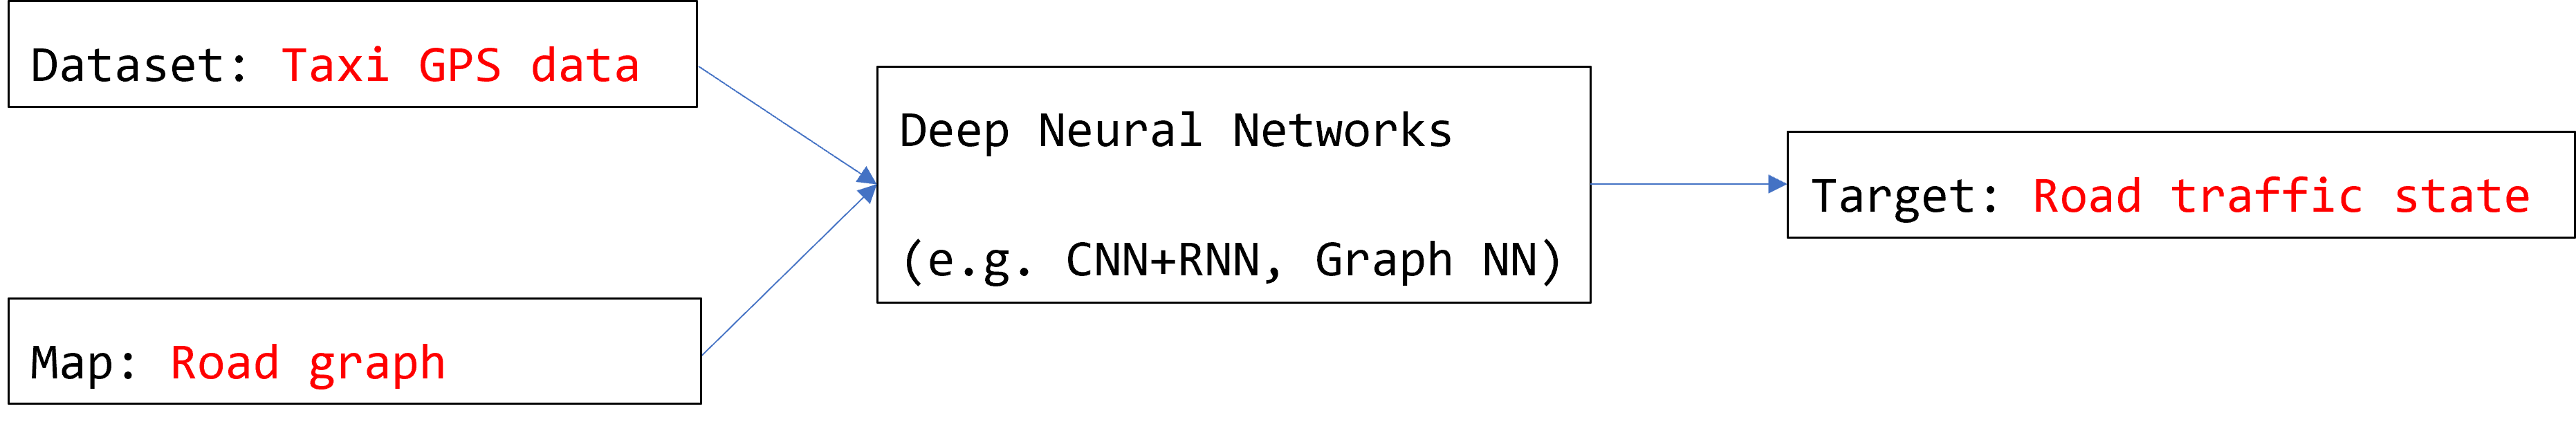
\includegraphics[width=\textwidth]{images/mid/1-2.png}
  \caption{Workflow of traffic prediction}
  \label{fig: 1-2}
\end{figure}

\begin{figure}[htb]
  \centering
  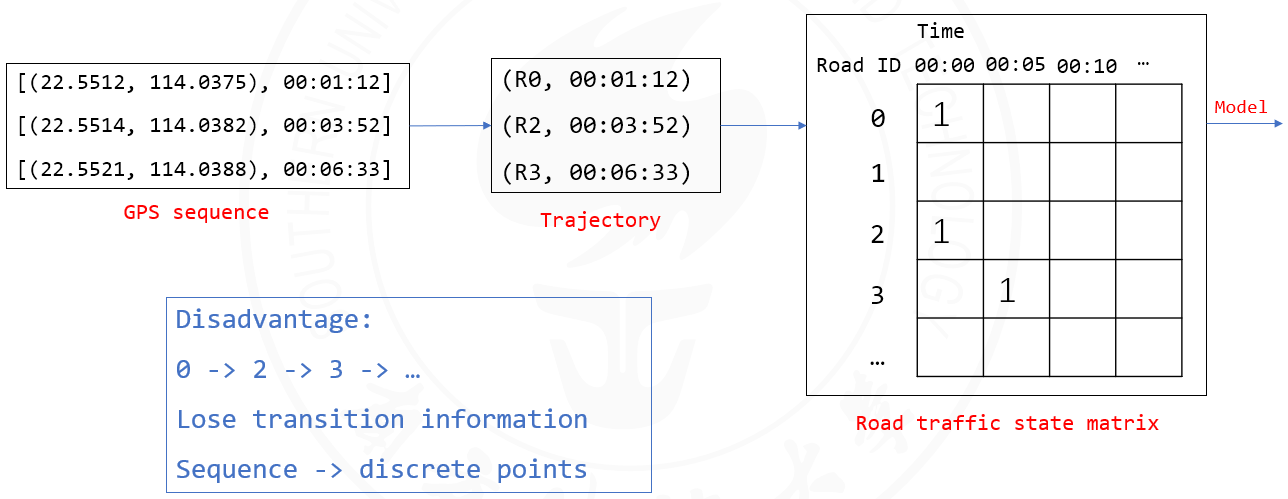
\includegraphics[width=\textwidth]{images/mid/1-3.png}
  \caption{Input Data}
  \label{fig: 1-3}
\end{figure}

\subsection{Work Plan}
The basic design and plan is shown in the following figure:

\begin{figure}[htb]
  \centering
  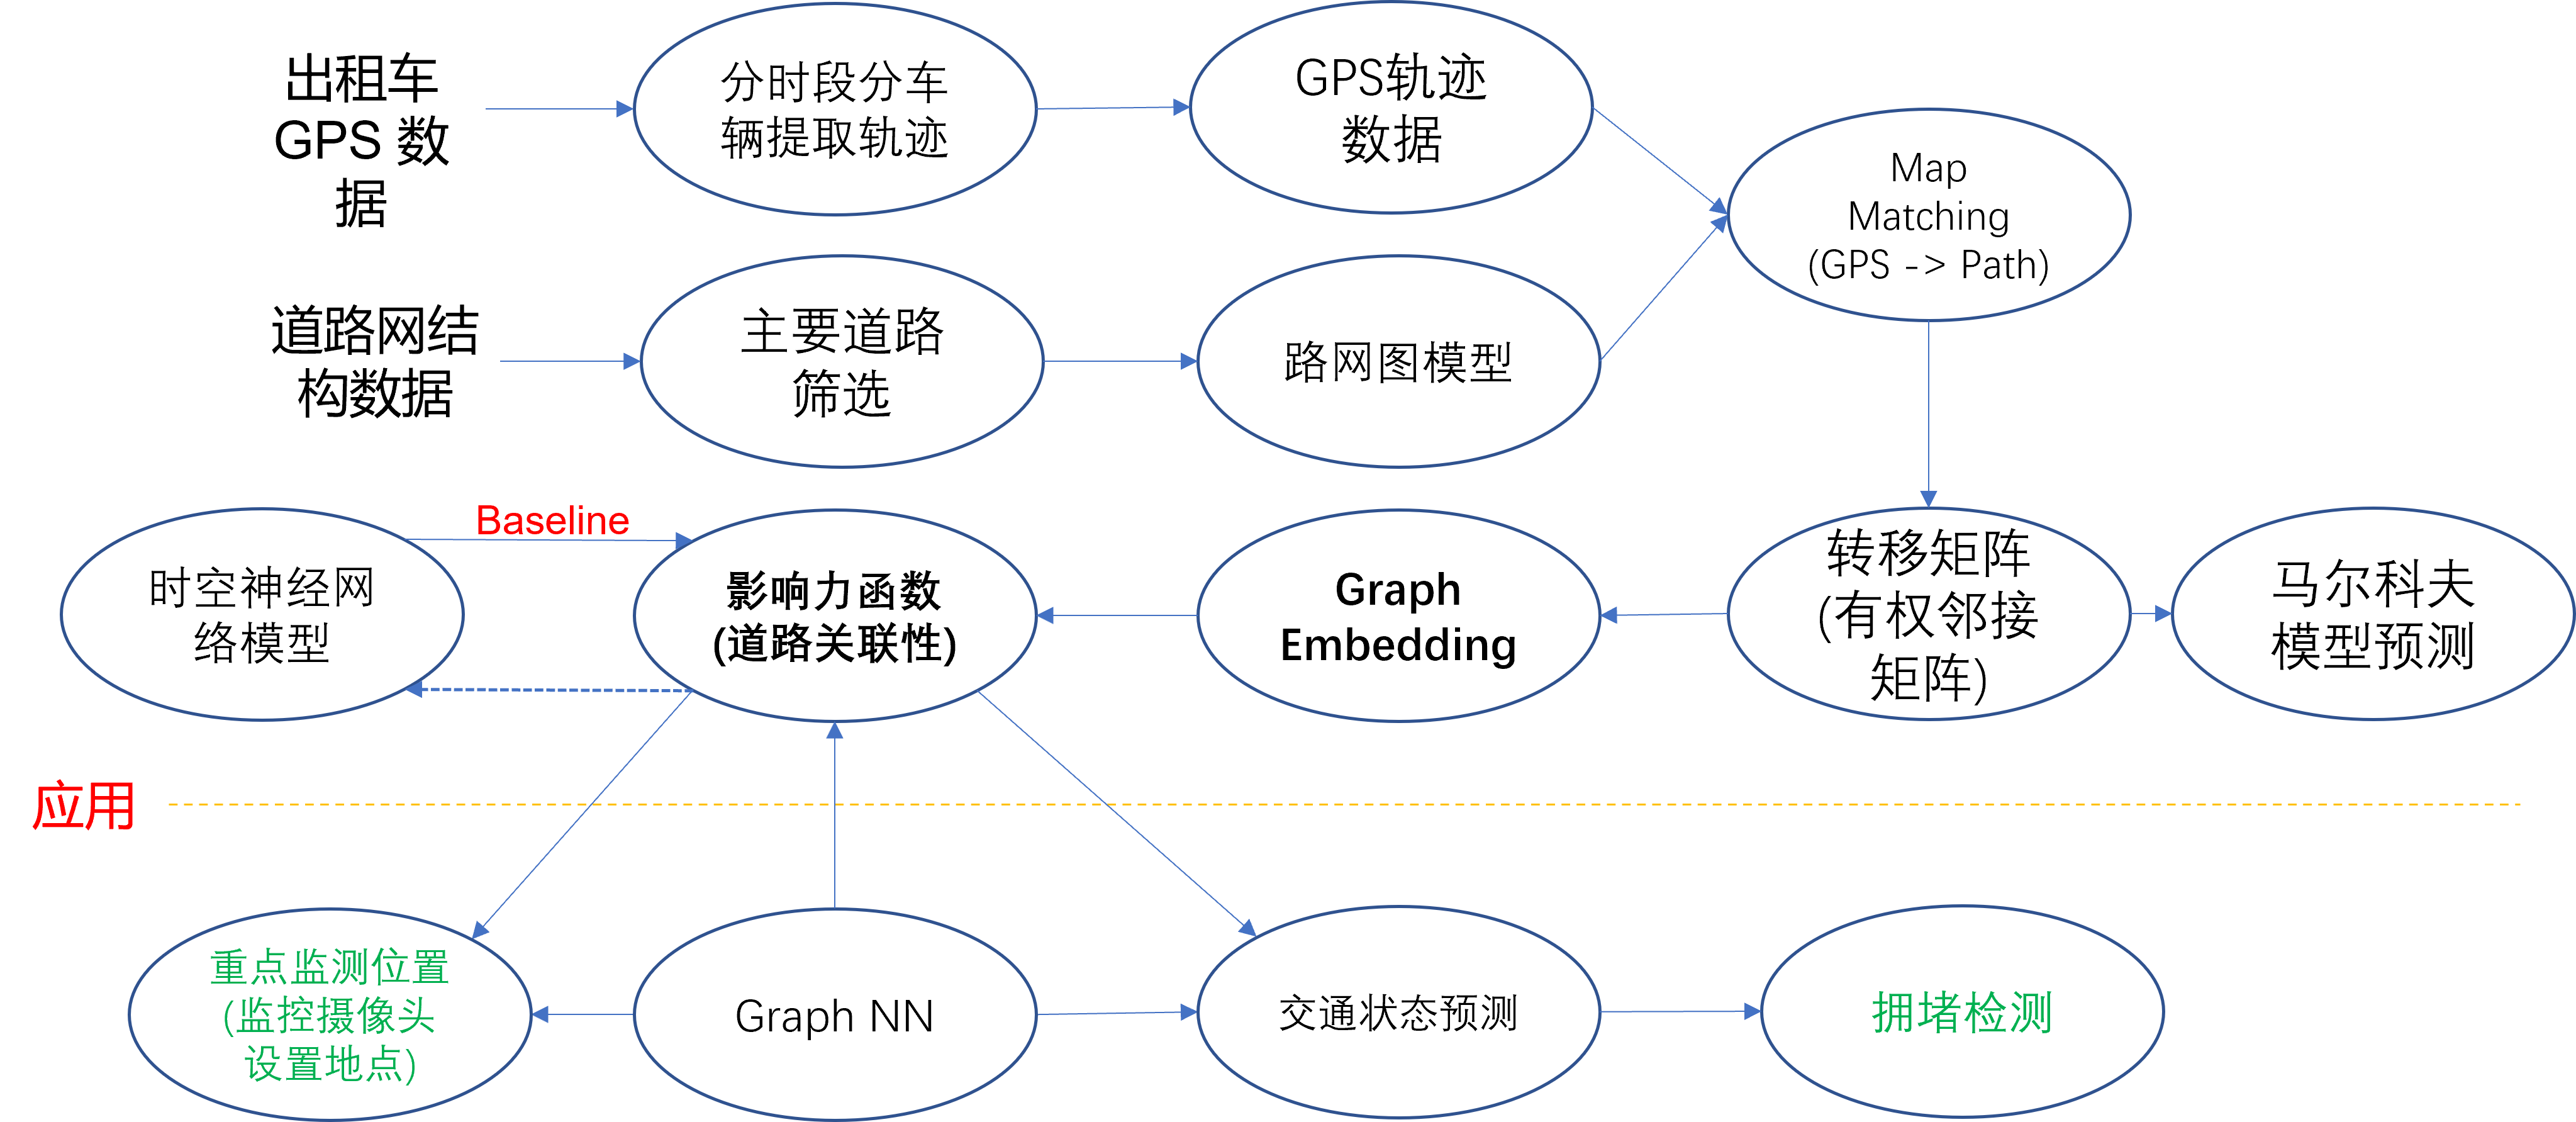
\includegraphics[width=\textwidth]{images/mid/plan.png}
  \caption{Plan}
  \label{fig: plan}
\end{figure}

\begin{enumerate}
  \item Process taxi GPS data to get tracks
  \item Process road network data to get a basic graph model
  \item Match tracks to each road and get the adjacent matrix of the graph
  \item Try a simple prediction based on Markov model
  \item \textbf{Graph embedding}
  \item \textbf{Influence function design}
  \item Combine spatial-temporal models and use them as baseline
  \item Embed road influence function into graph neural networks to predict traffic states
  \item Future Applications: traffic surveillance camera position and traffic jam detection
\end{enumerate}

\clearpage
\section{Dataset and Data Processing}
\subsection{Overview}
In traffic prediction area, the mostly used datasets are traffic sensor datasets.
Traffic sensors can detect road traffic flow and average speed.
Therefore, it can be directly entered into deep neural network models.
In recent studies, most of the traffic state prediction models use sensor data.
On the contrary, GPS data needs a series of data processing methods, which makes it hard to use.

\subsection{Data Description}
\begin{itemize}
  \item Region: Shenzhen
  \item Time: 2020-06
  \item Content: Taxi trajectory data
    \begin{itemize}
      \item License number
      \item Longitude and latitude
      \item Speed
      \item Timestamp
    \end{itemize}
  \item Size: Over 2,700,000,000 rows
\end{itemize}

\begin{figure}[htb]
  \centering
  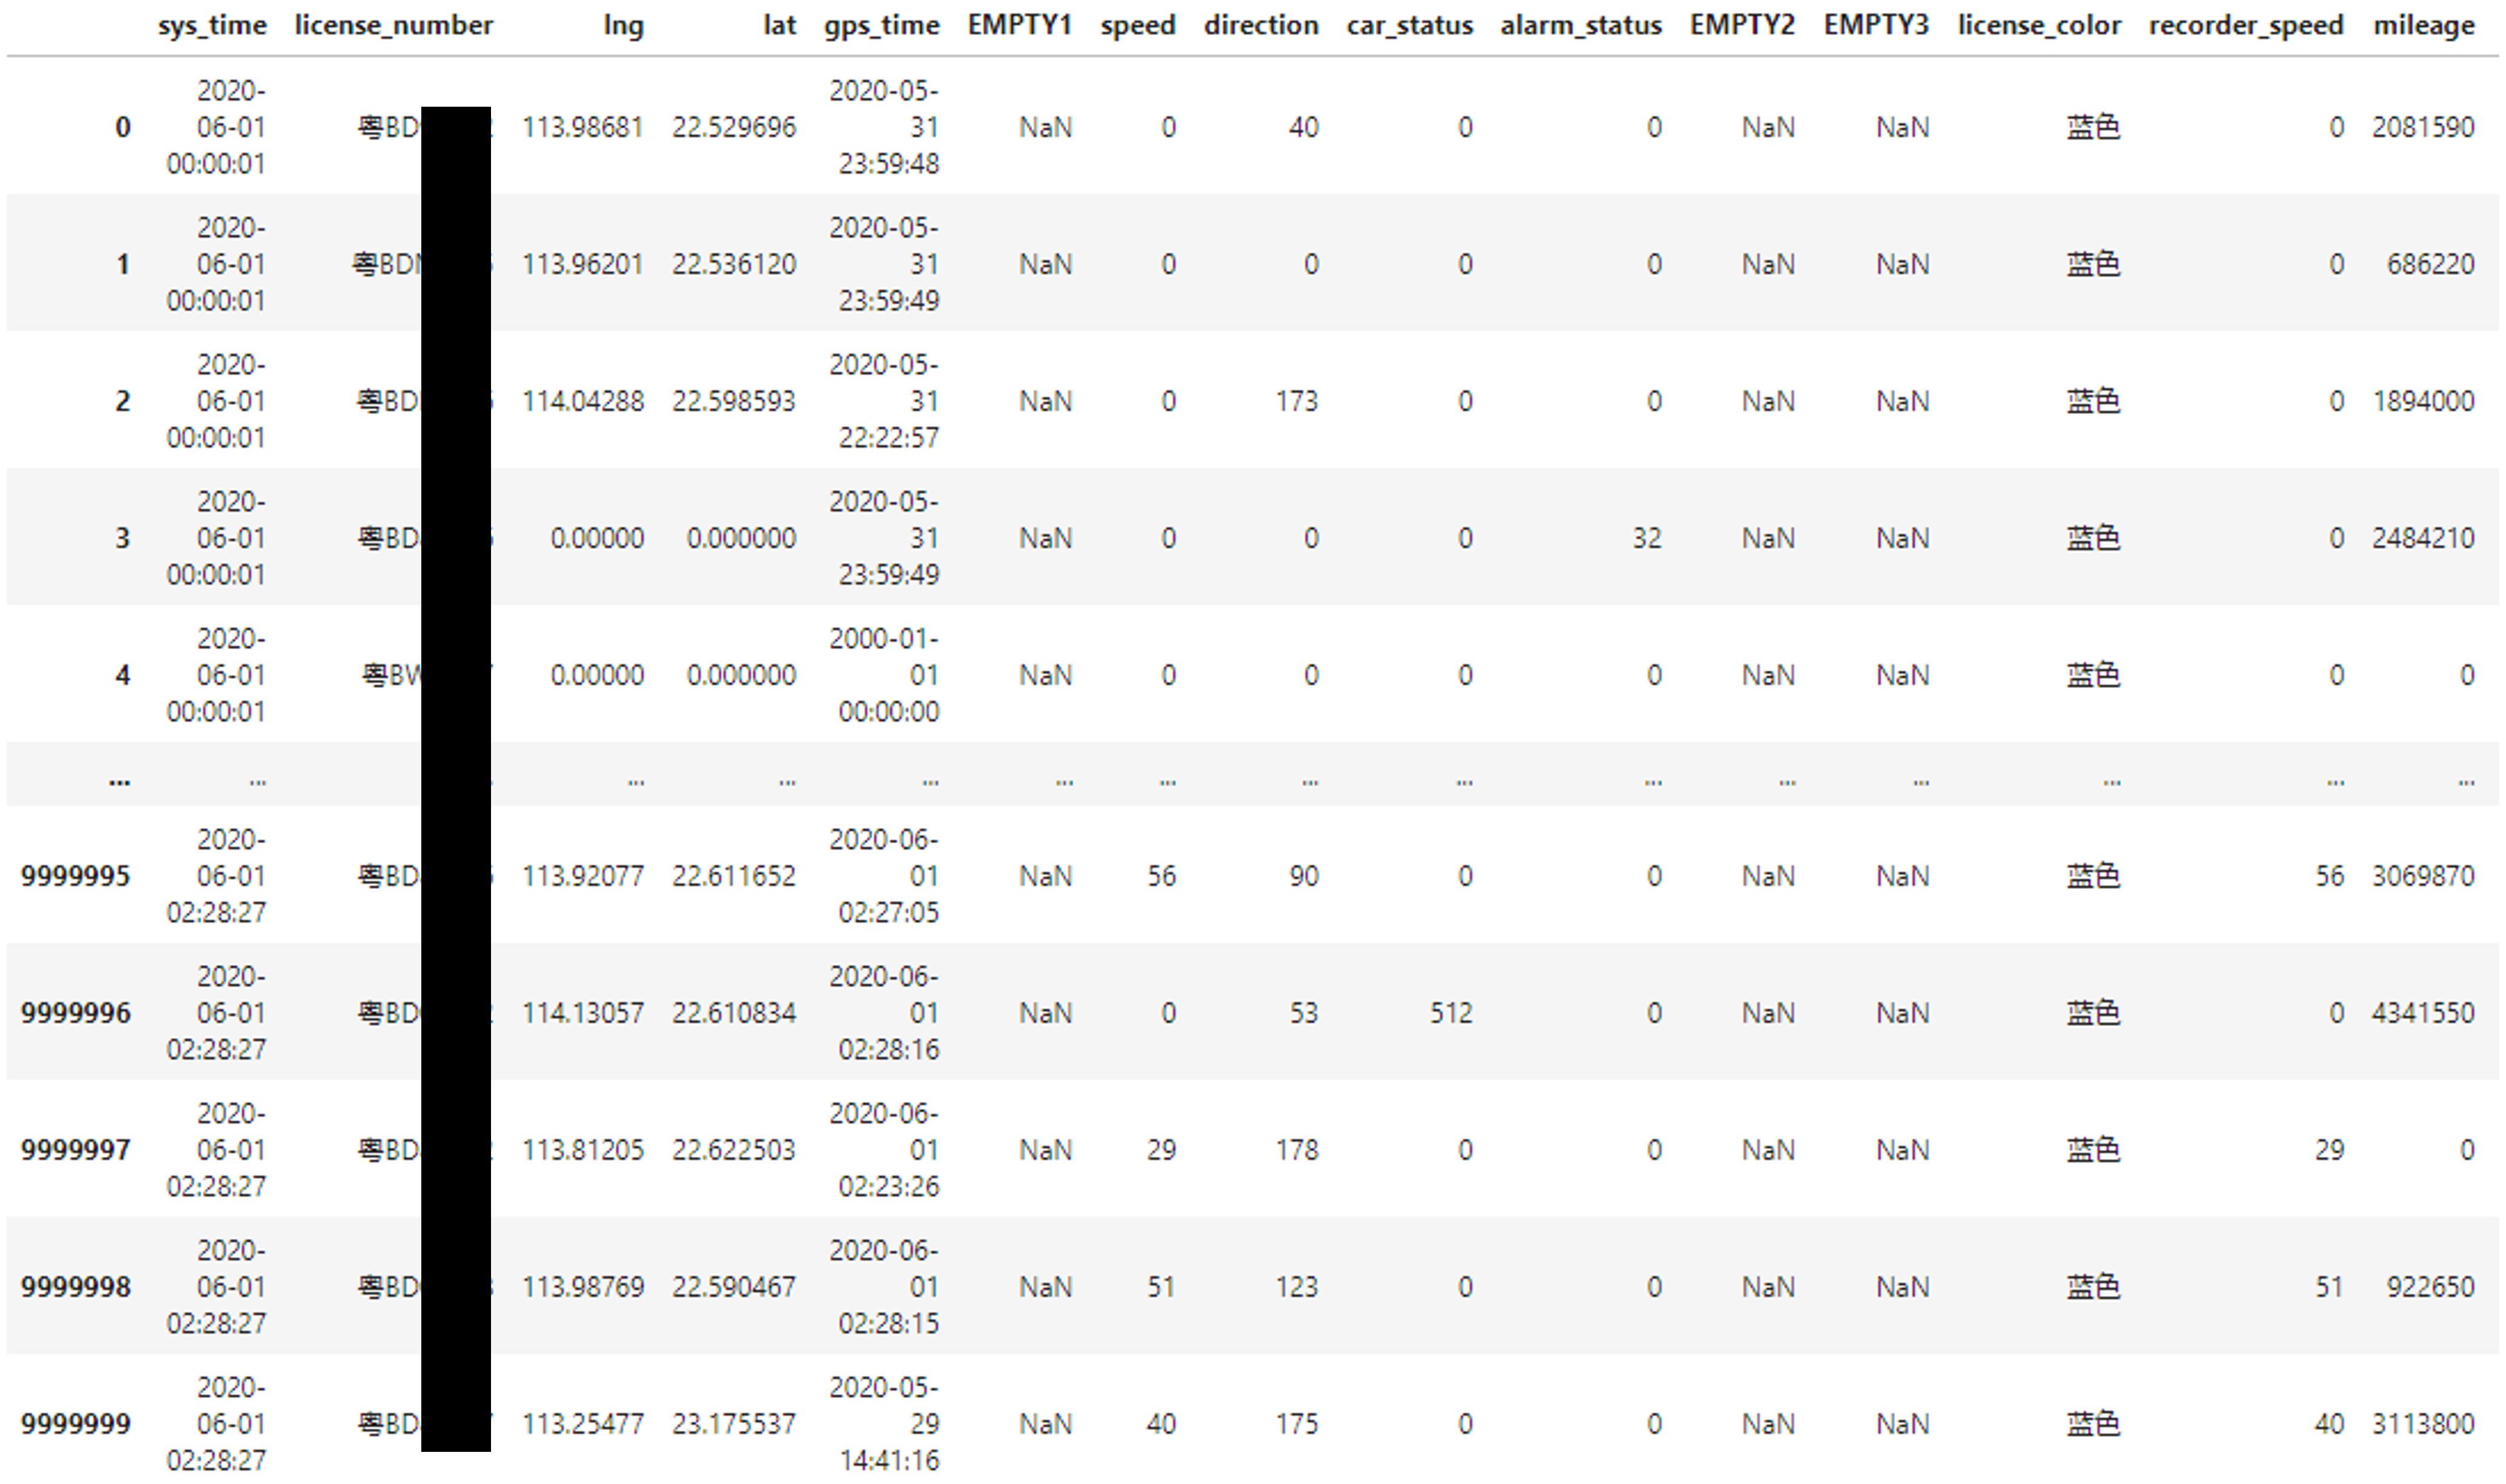
\includegraphics[width=\textwidth]{images/mid/2-1.png}
  \caption{Shenzhen Taxi GPS Raw Dataset}
  \label{fig: 2-1}
\end{figure}

In contrast to those open datasets, we have a completely raw dataset which was taken directly
from the raw records in Transportation Bureau of Shenzhen. Unlike the open datasets that can be
applied to deep learning models without the need of data cleaning and completion, this raw dataset
contains lots of abnormal values, which should be cleaned and re-organized carefully.

\subsection{Data Cleaning}
Since the raw data contains plenty of noise, the first step is to clean the whole dataset.
\begin{enumerate}
  \item Drop duplicate
  \item Drop time not in 2020-06
  \item Drop latitude or longitude is 0
  \item Drop speed is 0 or too large because motionless data is useless
  \item Drop useless columns
\end{enumerate}

After that, we got $48\%$ rows deleted, around $1.3$ billon, which means the raw data is very dirty.
For example, the speed distribution before and after data cleaning is shown below:
\begin{figure}[h]
  \centering
  \subfigure[Before Cleaning] {
    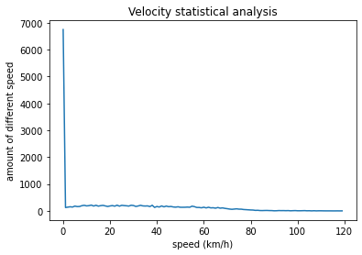
\includegraphics[width=0.45\textwidth]{images/mid/2-2.png}
  }
  \quad
  \subfigure[After Cleaning] {
    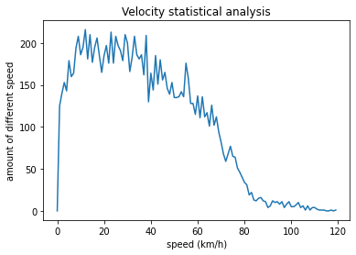
\includegraphics[width=0.45\textwidth]{images/mid/2-3.png}
  }
  \caption{Speed Distribution}
\end{figure}

\subsection{Data Processing}
As shown in figure \ref{fig: 2-4}, a GPS point mainly contains five attributes, which are
\texttt{(Taxi ID, Latitude, Longitude, Speed, Timestamp)}. First, we need to sort these GPS
points by timestamp for each taxi ID and get GPS sequences.

\begin{figure}[htb]
  \centering
  \subfigure[Map acquired via \textit{OSM} API] {
    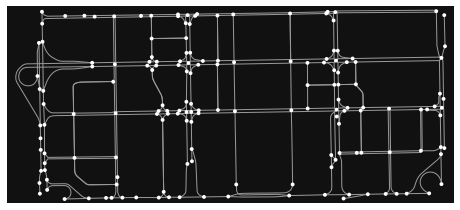
\includegraphics[width=0.45\textwidth]{images/mid/2-6.png}
    \label{fig: 2-6}
  }
  \quad
  \subfigure[Map after consolidating nodes] {
    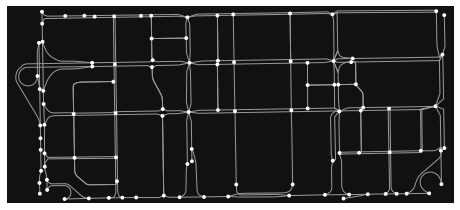
\includegraphics[width=0.45\textwidth]{images/mid/2-7.png}
    \label{fig: 2-7}
  }
  \caption{Road Map}
\end{figure}

To acquire trajectories, we need a road map that contains geometry information of roads.
\textit{OpenStreetMap (OSM)} is a collaborative project to create a free editable geographic database of the world.\cite{haklay2008openstreetmap}
It is easy require map data via its API by \textit{OSMnx} library in \textit{Python}. Since Shenzhen is a
big city, we chose a rectangle part of roads in CBD, which is shown in figure \ref{fig: 2-6}. The return type of
the map is \texttt{networkx.MultiDiGraph} that can be used and analyzed directly in \textit{Python} code.
In addition, as we can see in the figure, the original \textit{OSM} map has lots of nodes that can be
consolidated, typically on road intersections. Map simplification is another big research topic in 
Geographic Information System (GIS) area. A simple way here is to use built-in library functions or just
draw manually. The road map after simplification is shown in figure \ref{fig: 2-7}.

\begin{figure}[htb]
  \centering
  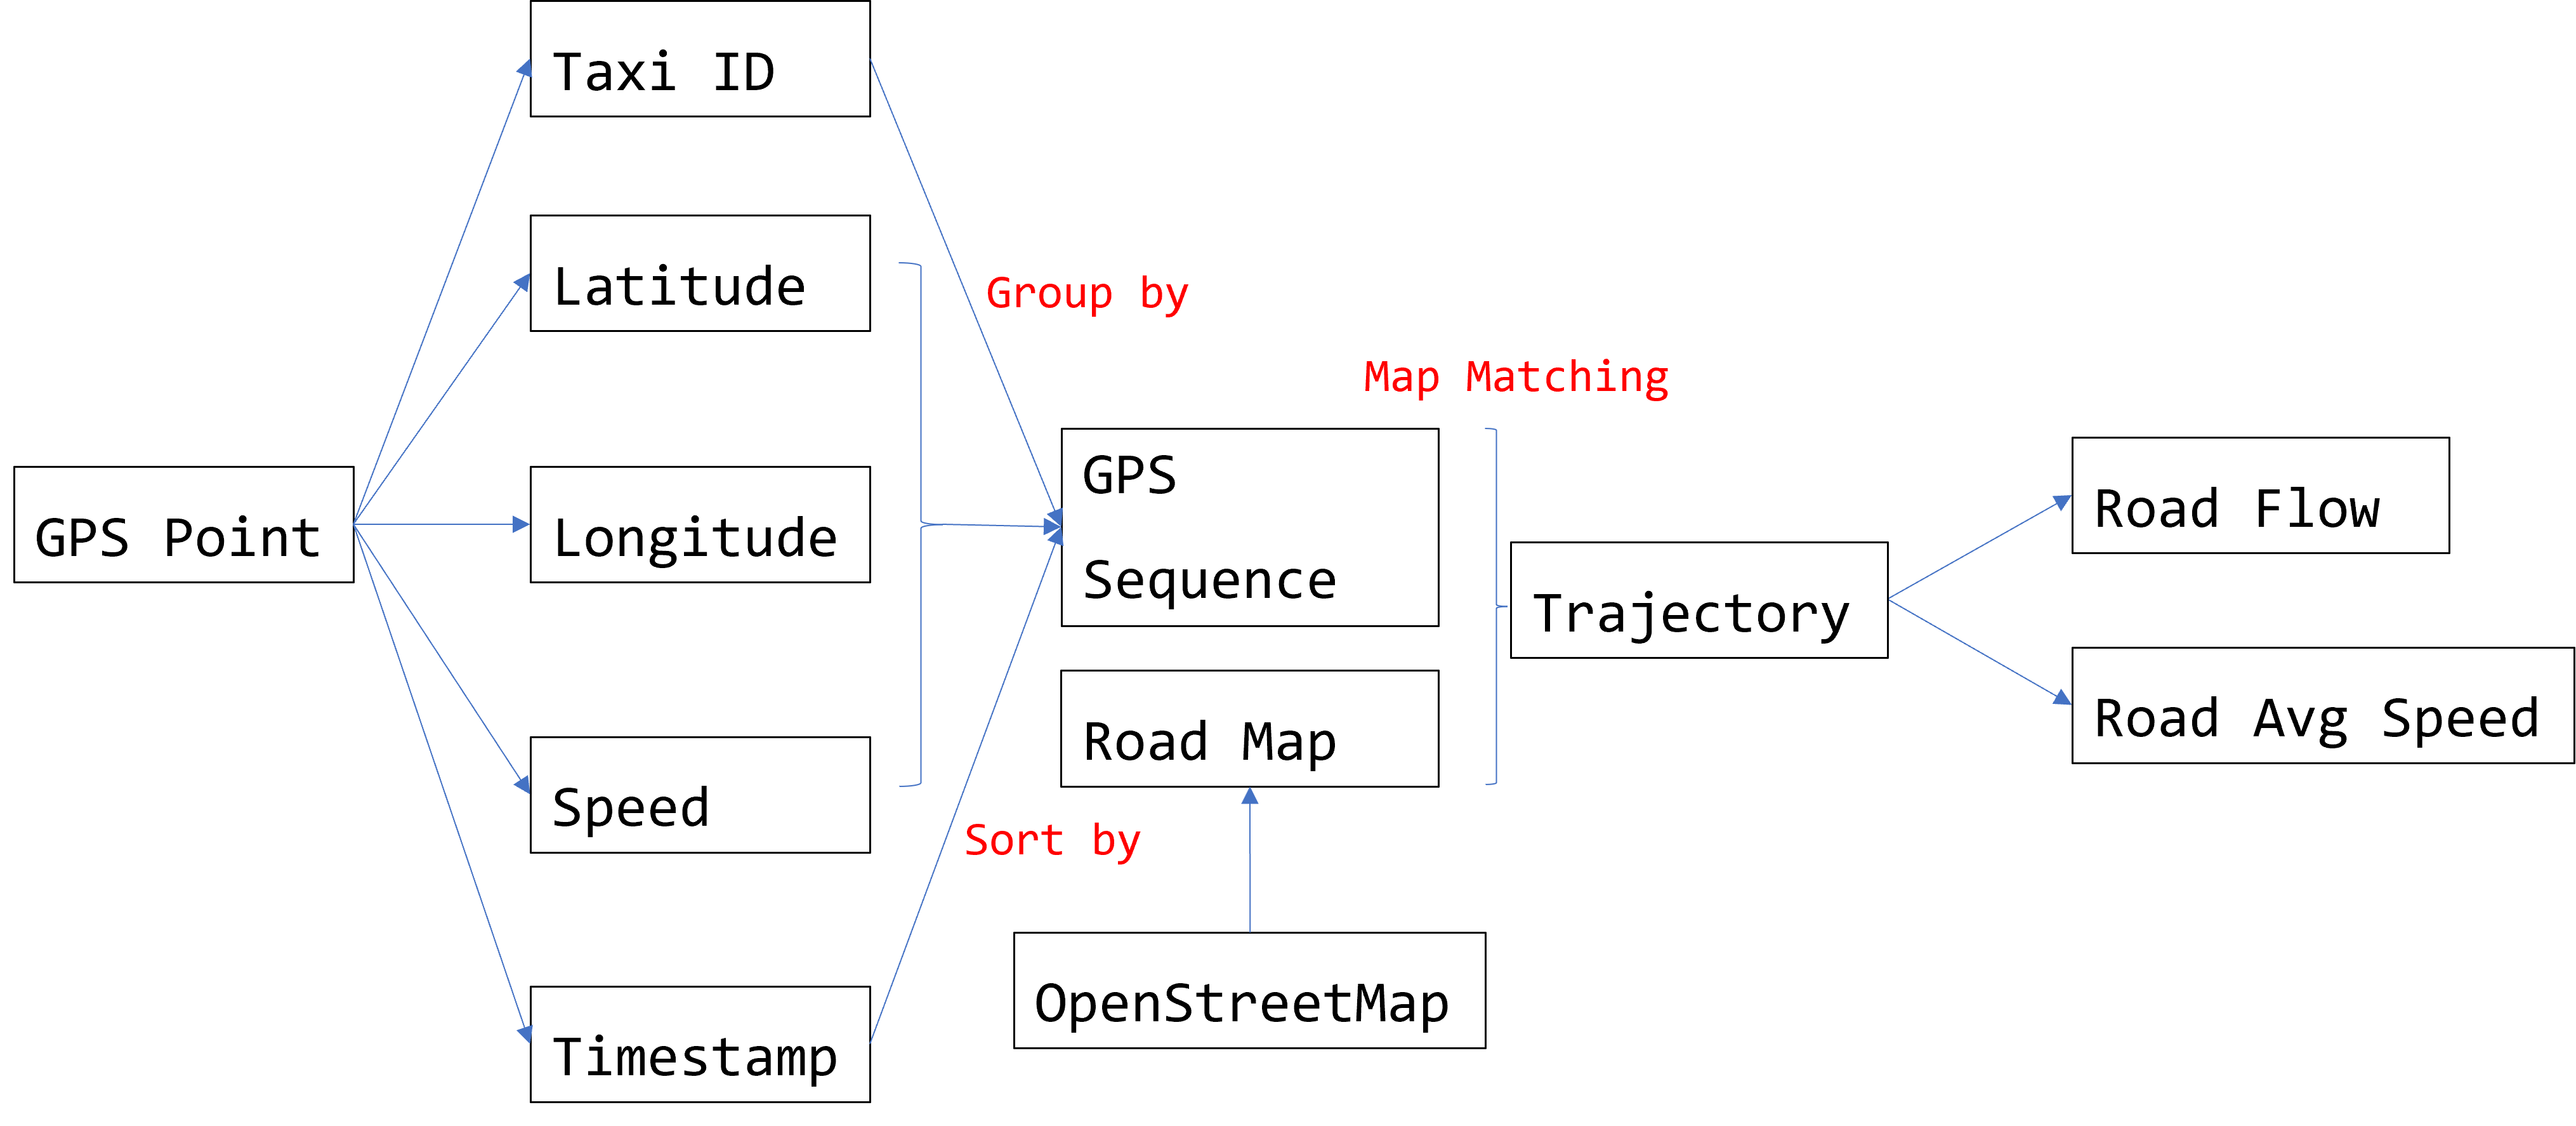
\includegraphics[width=\textwidth]{images/mid/2-4.png}
  \caption{Data Processing Pipeline}
  \label{fig: 2-4}
\end{figure}

Breifly, a trajectory refers to a path in road map, which is a sequence of road IDs in particular.
For example, a GPS sequence can be $[(22.551, 114.012), (22.562, 114.023), (22.569, 114.024)]$, and
the corresponding trajectory is $[Road_{3}, Road_{12}, Road_{24}]$.
The next step is to combine GPS sequences and road map to get trajectories.
Therefore, to decide a GPS point is on which road, we need \textbf{Map Matching}.
Map matching is the problem of how to match recorded geographic coordinates to a logical model of the real world.
The most common approach is to take recorded, serial location points (e.g. from GPS) and relate them to edges in an existing street graph (network), usually in a sorted list representing the travel of a user or vehicle.
\textit{Fast Map Matching (FMM)}\cite{Yang2018FastMM} is an open source map matching framework in \textit{C++} and \textit{Python}. It solves the problem of matching noisy GPS data to a road network.
The output example of \textit{FMM} is shown in figure \ref{fig: 2-8}.

The last step is counting traffic flow and calculating average speed on each road.
We aggregate traffic flow and speed on each 5 minutes.
With trajectory data, it is easy to do this by a for-loop and increment.
The final representaion of processed data is given in figure \ref{fig: 2-9}, and we call the form
as ``stacked vector''\cite{lee2021short}. After that, we can put it into some baseline models to get a basic result.

\clearpage
\begin{figure}[t]
  \centering
  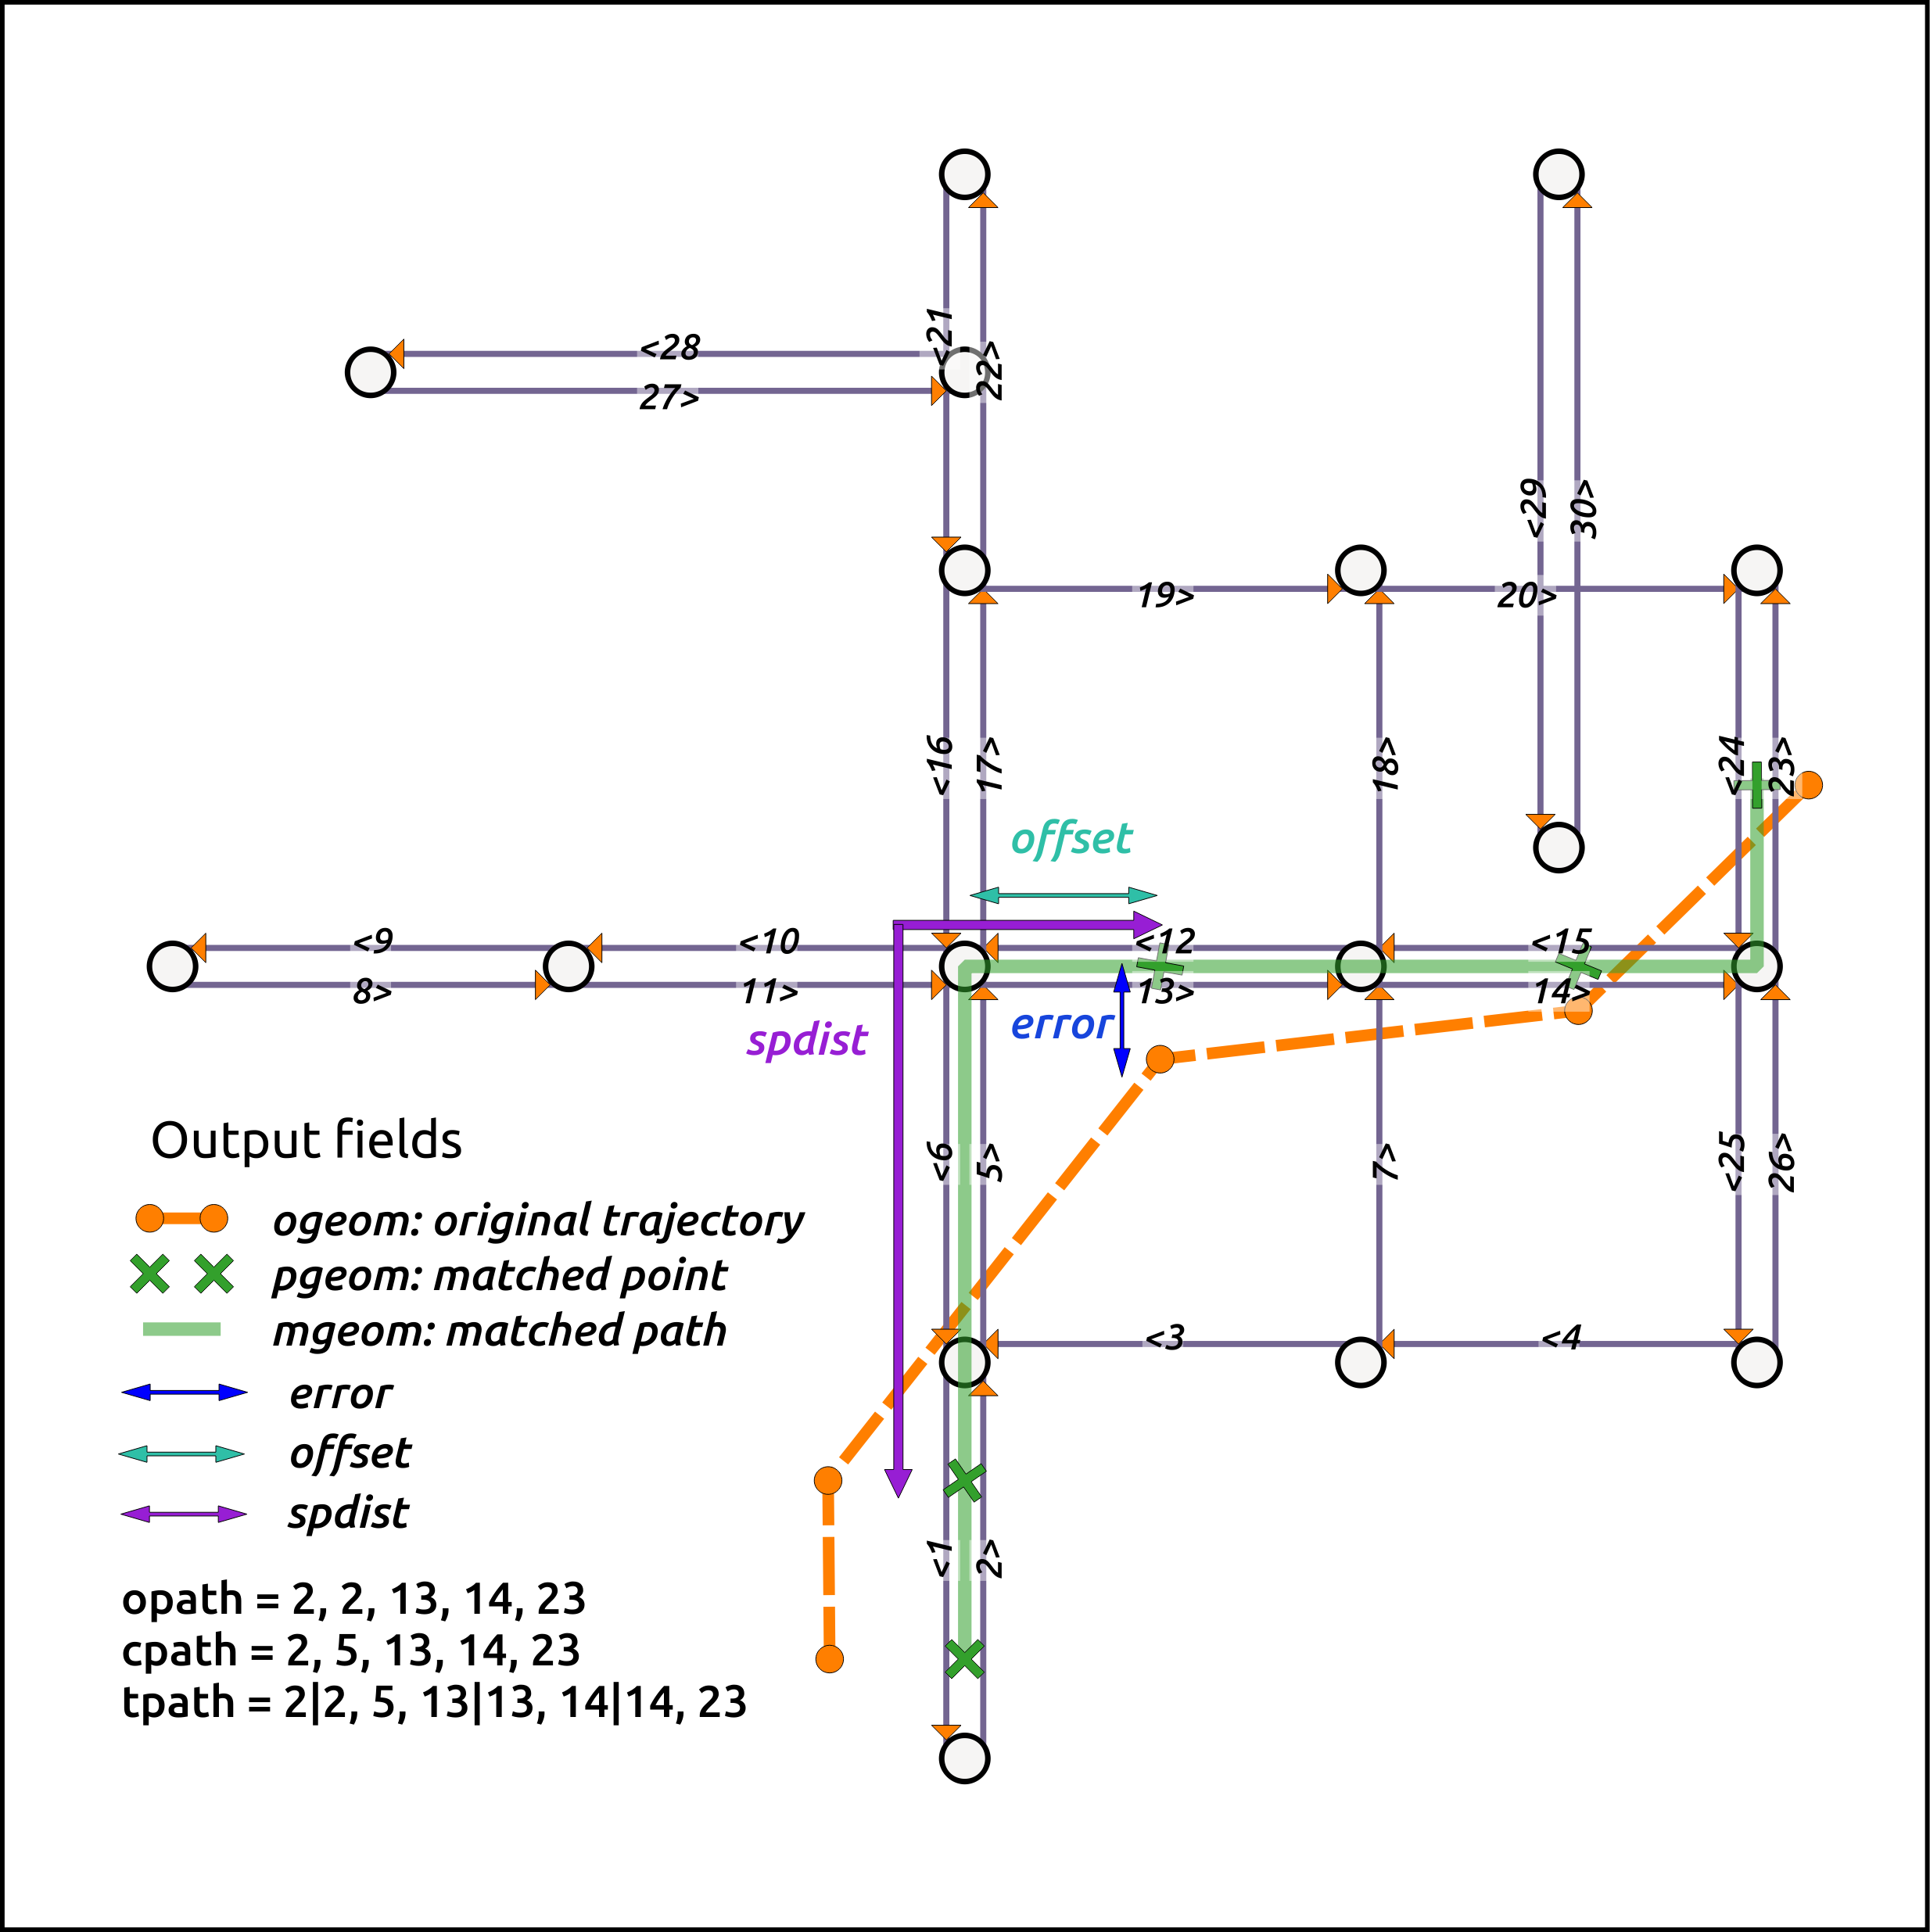
\includegraphics[width=0.8\textwidth]{images/mid/2-8.png}
  \caption{\textit{Fast Map Matching (FMM)}}
  \label{fig: 2-8}
\end{figure}

\begin{figure}[b]
  \centering
  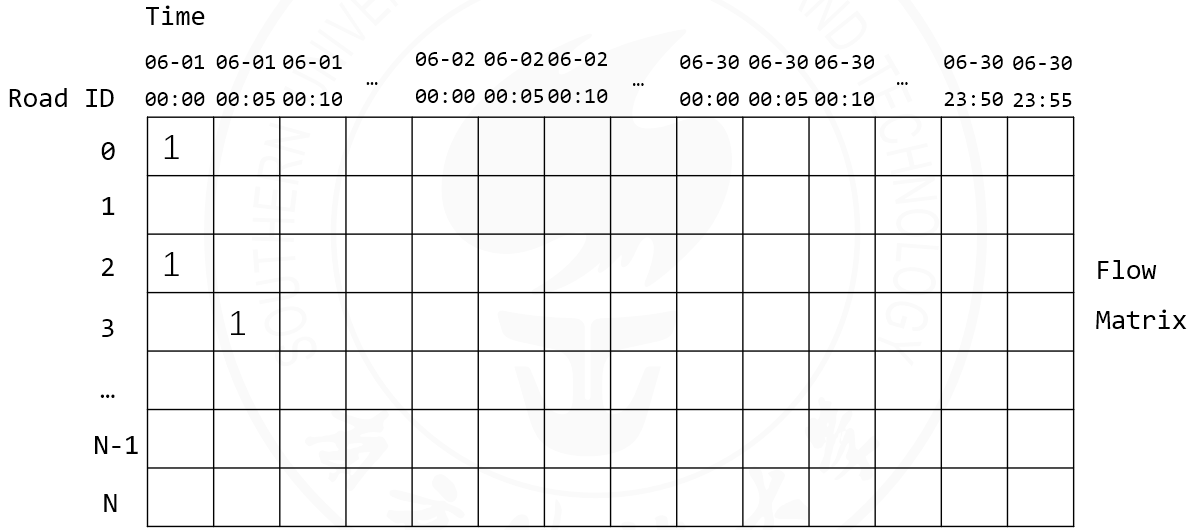
\includegraphics[width=0.8\textwidth]{images/mid/2-9.png}
  \caption{Stacked Vector}
  \label{fig: 2-9}
\end{figure}

\clearpage
\section{Baseline Experiment}
In this section, we tried several SOTA models to test the quality of our dataset.
\begin{itemize}
  \item AGCRN, NeurIPS 2020\cite{bai2020adaptive}
  \item Graph WaveNet, IJCAI 2019\cite{wu2019graph}
  \item LSTNet, SIGIR 2018\cite{lai2018modeling}
  \item MTGNN, SIGKDD 2020\cite{wu2020connecting}
  \item STNorm, SIGKDD 2021\cite{deng2021st}
\end{itemize}

To evaluate the accuracy of the simulation
results, we calculated prediction error with three different
metrics, which are mean absolute error (MAE),
masked mean absolute percentage error (Masked MAPE), and root-mean-square error
(RMSE). They are defined as:

\begin{equation}
  MAE=\frac 1n\sum_{i=1}^n|\hat{y_i}-y_i|\notag
\end{equation}

\begin{equation}
  Masked\ MAPE=\frac 1n\sum_{i=1}^n|\frac{\hat{y_i}-y_i}{y_i}|, y_i\neq 0 \notag
\end{equation}

\begin{equation}
  RMSE=\sqrt{\frac 1n\sum_{i=1}^n(\hat{y_i}-y_i)^2}\notag
\end{equation}

We have compared the performance of the baselines.
The left half of table \ref{tab: eval} shows the evaluation result of traffic flow prediction.
Our dataset has a low MAE and RMSE on these baseline models, but MAPE is a little high
compared to traffic sensors datasets. This is because baselines are designed for sensor data,
i.e. trajectory data are seldomly used in traffic state forecasting area, which is a challenge to us.

And the right half of table \ref{tab: eval} shows the result of road average speed prediction. MAPE is much lower but still
higher than traffic sensor datasets (e.g. SOTA models can reach less than $10\%$ MAPE on METR-LA dataset).
We consider that it is because our data cleaning process makes the sampling frequency lower than the normal case.
And it should be improved in the future.

\begin{table}[htb]
  \centering
  \begin{tabular}{c|c|c|c||c|c|c}
  \hline\hline
      \multirow{2}{*}{Model} & \multicolumn{3}{c||}{Flow} & \multicolumn{3}{c}{Speed} \\ \cline{2-7}
      ~ & MAE & M MAPE & RMSE & MAE & M MAPE & RMSE \\ \hline
      AGCRN & 3.409 & 0.332 & 4.37 & 4.642 & 0.238 & 6.587 \\
      GWNET & 3.478 & 0.344 & 4.791 & 4.714 & 0.242 & 6.666 \\
      LSTNet & 3.648 & 0.35 & 4.819 & 4.914 & 0.247 & 6.81 \\
      MTGNN & 3.35 & 0.327 & 4.279 & 4.649 & 0.237 & 6.593 \\
      STNorm & 3.303 & 0.323 & 4.233 & 4.637 & 0.238 & 6.576 \\ \hline
  \end{tabular}
  \caption{Evaluation Results}
  \label{tab: eval}
\end{table}

\clearpage
\phantomsection
\addcontentsline{toc}{section}{References}
\bibliographystyle{ieeetr}
\bibliography{references-mid}

\end{document}